% !TEX program = xelatex
% DGMAE Presentation — CS313 R11
% Compile with: xelatex main.tex

\documentclass[aspectratio=169,10pt]{beamer}

% ── Giao diện (Madrid + beaver, font Latin Modern Sans) — xem theme.tex ──
% ══════════════════════════════════════════════════════
% Giao diện theo mẫu slide môn học (CS313 — Course Overview):
% Beamer Madrid + colortheme beaver (đỏ đậm trên nền xám), font Latin Modern Sans
% (bản OpenType của Computer Modern Sans, có đủ dấu tiếng Việt). Biên dịch bằng XeLaTeX.
% ══════════════════════════════════════════════════════

\usetheme{Madrid}
\usecolortheme{beaver}
\usepackage{tikz}   % theme cũ (Durham) tự nạp TikZ; phần 1 có dùng

% ── Font: Latin Modern Sans (nạp theo tên file để chạy được cả trên Overleaf lẫn máy cá nhân) ──
\usepackage{fontspec}
\setsansfont{lmsans10-regular.otf}[
  BoldFont       = lmsans10-bold.otf,
  ItalicFont     = lmsans10-oblique.otf,
  BoldItalicFont = lmsans10-boldoblique.otf]
\setmonofont{lmmono10-regular.otf}

% ── Tên màu cũ vẫn được các phần slide dùng → ánh xạ sang bảng màu mới ──
\colorlet{Theme_Color}{darkred}             % màu nhấn chính (đỏ của beaver)
\colorlet{RiverDark}{darkred!80!black}      % đỏ đậm
\colorlet{RiverLight}{gray!10}              % nền xám nhạt (giống nền tiêu đề slide)
\colorlet{RiverAccent}{darkred!50}

% ── Block: Madrid mặc định dùng tiêu đề xanh navy → đổi sang tông đỏ/xám cho khớp beaver ──
\setbeamercolor{block title}{fg=white, bg=darkred!80!black}
\setbeamercolor{block title alerted}{fg=white, bg=darkred}
\setbeamercolor{block title example}{fg=white, bg=gray!60!black}
\setbeamercolor{block body}{bg=gray!8}
\setbeamercolor{block body alerted}{bg=gray!8}
\setbeamercolor{block body example}{bg=gray!8}

% ── Trang phân mục & các slide dùng chung ──
\renewcommand{\sectionname}{Phần}
\AtBeginSection[]{\begin{frame}\sectionpage\end{frame}}
\newcommand{\makeoutline}{\begin{frame}{Nội dung}\tableofcontents\end{frame}}
\newcommand{\makethankyou}{%
  \begin{frame}
    \centering\vfill
    {\usebeamercolor[fg]{title}\Large Cảm ơn thầy cô và các bạn!}\\[1em]
    Câu hỏi · Góp ý · Thảo luận
    \vfill
  \end{frame}}


% ── Toán & ký hiệu ──
\usepackage{amsmath,amssymb}
\usepackage{mathtools}
\usepackage{bm}

% ── Đồ họa & bảng ──
\usepackage{graphicx}
\graphicspath{{1-intro/figures/}{2-method/figures/}{3-experiment/figures/}{figures/}}
\usepackage{booktabs}
\usepackage{multirow}
\usepackage{adjustbox}

% ══════════════════════════════════════════════════════
% Metadata bài thuyết trình
% ══════════════════════════════════════════════════════
\title[DGMAE · Data Mining]{Discrepancy-Aware Graph Mask Auto-Encoder (DGMAE)}
\subtitle{}
\author[Group 2]{%
  Group 2\\[0.6em]
  {\footnotesize
  \begin{tabular}{@{}l@{\hspace{0.8em}}l@{\hspace{2.5em}}l@{\hspace{0.8em}}l@{}}
    Đặng Phú Duy        & 24520010 & Trịnh Duy Hưng        & 24520015 \\
    Đoàn Hồng Bảo       & 24520005 & Lương Huỳnh Gia Bảo   & 24520006 \\
    Nguyễn Trường Giang & 24520011 & Trần Xuân Đạt         & 24520008 \\
                        &          & Trần Nguyễn Khải Lạc  & 24520018 \\
  \end{tabular}}}
\institute[UIT]{CS313 - Data Mining and Application}
\date{Nov 22, 2026}

% ══════════════════════════════════════════════════════
\begin{document}

% ── Slide tiêu đề (kèm thành viên & MSSV) ──
\maketitle

% ── Giới thiệu đề tài ──
\begin{frame}{Giới thiệu đề tài}
  \begin{columns}[c]
    \begin{column}{0.50\textwidth}
      \textbf{Môn:} Data Mining \\[0.4em]
      \textbf{Paper:} Discrepancy-Aware Graph Mask Auto-Encoder (DGMAE) \\
      {\small Ziyu Zheng, Yaming Yang, Ziyu Guan, Wei Zhao, Weigang Lu} \\
      {\small \textbf{KDD 2025} · arXiv:2506.19343}
      \vspace{0.6em}
      \begin{itemize}
        \item \textbf{Bài toán:} học biểu diễn node \textbf{không cần nhãn}
        \item \textbf{Vấn đề:} GMAE làm các node láng giềng \textbf{giống nhau}, kém trên đồ thị dị tính
        \item \textbf{Ý tưởng:} tái tạo thêm \textbf{sự khác biệt} (discrepancy) giữa node và láng giềng
      \end{itemize}
    \end{column}
    \begin{column}{0.46\textwidth}
      \centering
      \begin{tikzpicture}[
        scale=1.05,
        node_a/.style={circle, fill=Theme_Color!70, draw=Theme_Color, text=white, inner sep=0pt, minimum size=17pt, font=\scriptsize\bfseries},
        node_b/.style={circle, fill=orange!80, draw=orange!90!black, text=white, inner sep=0pt, minimum size=17pt, font=\scriptsize\bfseries},
        node_mask/.style={circle, fill=white, draw=Theme_Color, dashed, line width=1.1pt, text=Theme_Color, inner sep=0pt, minimum size=21pt, font=\small\bfseries},
        edge_homo/.style={thick, gray!55},
        edge_hetero/.style={very thick, orange!85!black, dashed}
      ]
        \node[node_mask] (vm) at (0, 0.1) {$?$};
        \node[node_a] (v1) at (-1.4, 1.2) {$v_1$};
        \node[node_a] (v2) at (-1.5, -0.9) {$v_2$};
        \node[node_b] (v3) at (1.5, 0.9) {$v_3$};
        \node[node_b] (v4) at (1.4, -1.0) {$v_4$};
        \node[node_a] (v5) at (-2.5, 0.2) {$v_5$};
        \node[node_b] (v6) at (2.5, -0.1) {$v_6$};
        \draw[edge_homo] (vm) -- (v1) node[midway, left=2pt, text=black!70, font=\scriptsize] {Cùng lớp};
        \draw[edge_homo] (vm) -- (v2);
        \draw[edge_homo] (v1) -- (v5);
        \draw[edge_homo] (v2) -- (v5);
        \draw[edge_hetero] (vm) -- (v3) node[pos=0.35, above=4pt, text=orange!90!black, font=\scriptsize\bfseries] {Khác lớp};
        \draw[edge_hetero] (vm) -- (v4) node[pos=0.4, below left=1pt, text=orange!90!black, font=\scriptsize\bfseries] {$x_i^D$};
        \draw[edge_homo] (v3) -- (v6);
        \draw[edge_homo] (v4) -- (v6);
        \draw[edge_homo] (v3) -- (v4);
        \node[anchor=north, align=center, text width=6.2cm, font=\scriptsize, yshift=-0.4cm] at (0, -1.2) {
          \tikz\draw[Theme_Color, dashed, line width=0.9pt, fill=white] (0,0) circle (3pt); Nút bị che \quad
          \tikz\fill[Theme_Color!70] (0,0) circle (3pt); Cùng lớp \quad
          \tikz\fill[orange!80] (0,0) circle (3pt); Khác lớp \\
          \vspace{0.2em}
          \textcolor{Theme_Color}{\textbf{DGMAE}}: bảo toàn sự khác biệt ($x_i^D$) giữa các nút dị tính
        };
      \end{tikzpicture}
    \end{column}
  \end{columns}
  % Lời thoại: Nhóm trình bày paper DGMAE (KDD 2025). Ý chính trong 1 câu: GMAE học bằng cách tái tạo node bị che
  % từ láng giềng, nên trên đồ thị dị tính (láng giềng khác lớp) các node bị "đồng nhất hóa". DGMAE tái tạo thêm
  % phần khác biệt x_i^D giữa node và láng giềng để giữ lại thông tin đó.
\end{frame}

% ── Mục lục ──
\makeoutline

% ══════════════════════════════════════════════════════
% PHẦN 1 — Mở đầu, Nền tảng, Kiến trúc
% Người thuyết trình: A (TV2 — Đoàn Hồng Bảo)  ~8 min
% ══════════════════════════════════════════════════════
% ══════════════════════════════════════════════════════
% PHẦN 1 — MỞ ĐẦU, NỀN TẢNG, KIẾN TRÚC
% Người thuyết trình: A (TV2 — Đoàn Hồng Bảo)
% Phong cách: Tối giản (Minimum) — Keyword + Biểu tượng
% ══════════════════════════════════════════════════════

\section{Mở đầu \& Nền tảng}

% ── Slide 1: Bài toán thực tế ──────────────────────────
\begin{frame}{Bài toán thực tế: Dữ liệu dạng đồ thị}
  \vspace{0.2em}
  \begin{columns}[c]
    \begin{column}{0.50\textwidth}
      \centering
      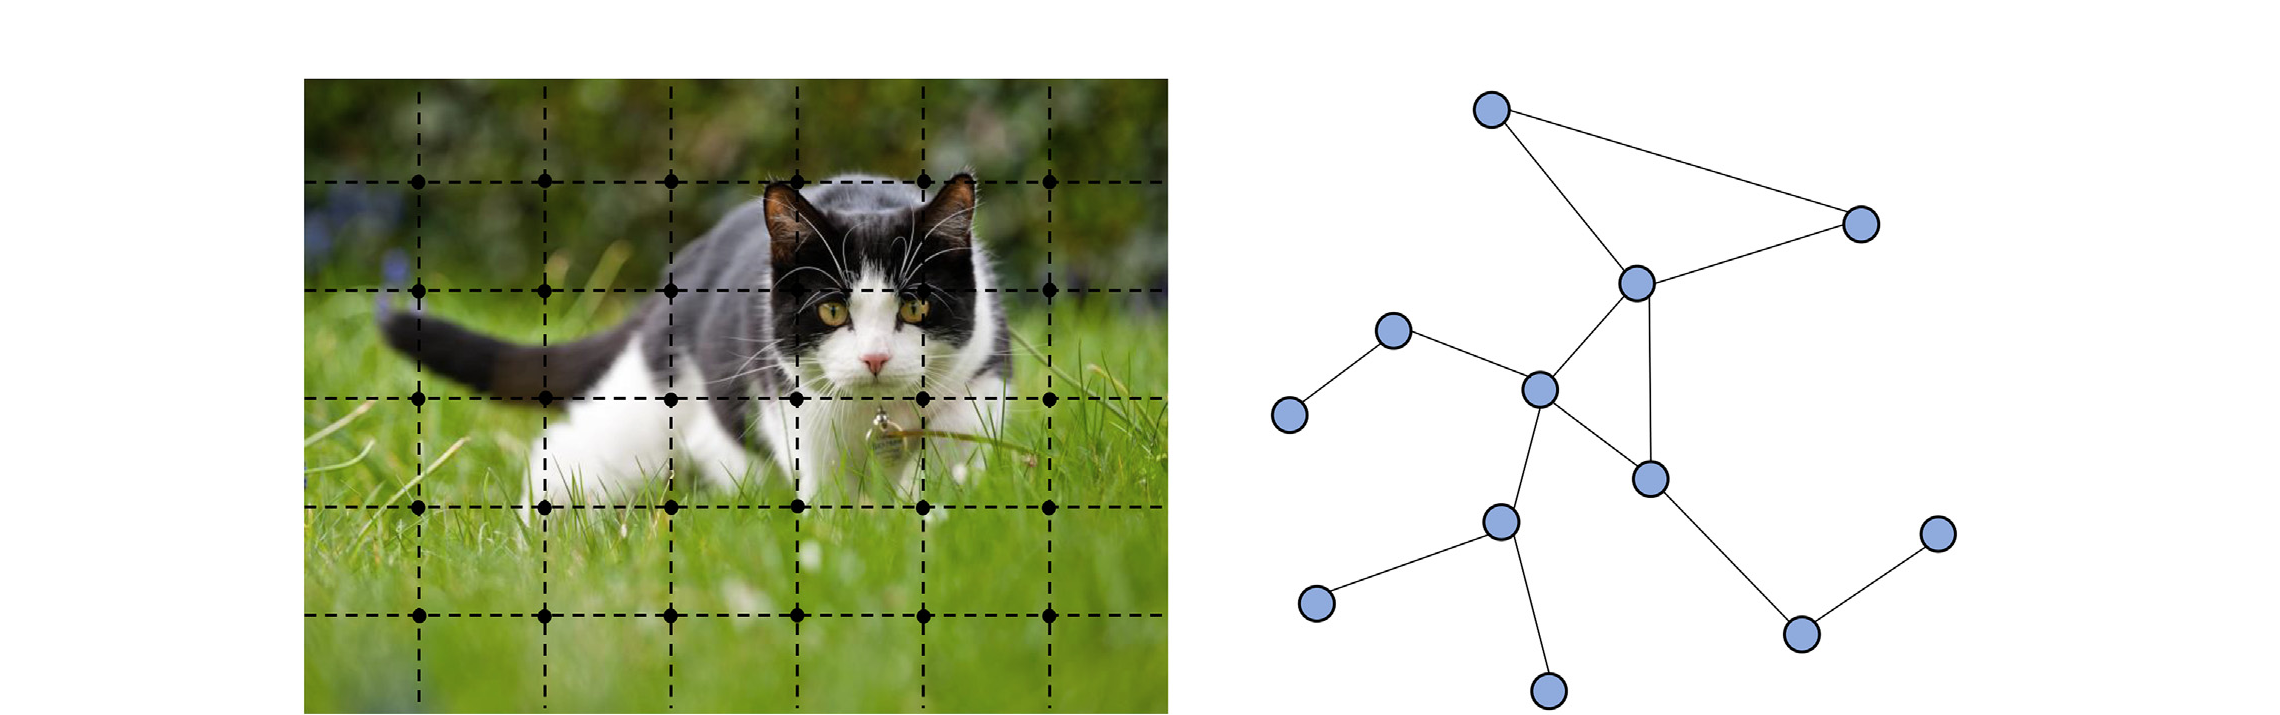
\includegraphics[width=\linewidth, height=0.36\textheight, keepaspectratio]{gnn/fig1_graph.png}
      \vspace{0.3em}

      {\footnotesize\textit{Zhou et al. (2020), Fig. 1: Ảnh (Euclidean) vs.\ Đồ thị (non-Euclidean)}}
    \end{column}

    \begin{column}{0.48\textwidth}
      \textcolor{Theme_Color}{\textbf{\large Ví dụ \& Bài toán}}
      \vspace{0.5em}
      \begin{itemize}
        \setlength{\itemsep}{0.5em}
        \item \textbf{Ví dụ:} Mạng xã hội $\cdot$ Mạng trích dẫn $\cdot$ Phân tử $\cdot$ Giao thông
        \item \textbf{Bài toán:} Phân loại nút — dự đoán nhãn từng nút
        \item \textbf{Thách thức:} Nhãn \textbf{đắt đỏ}, đồ thị \textbf{lớn} $\rightarrow$ thiếu dữ liệu giám sát
        \item \textcolor{orange!85!black}{\textbf{Hệ quả:}} Học biểu diễn \textbf{không giám sát} $\rightarrow$ \textbf{SSL}
      \end{itemize}
    \end{column}
  \end{columns}
\end{frame}


% ── Slide 2: Bài toán Đồ thị & SSL ─────────────────────
\begin{frame}{Bài toán Đồ thị \& Học tự giám sát (SSL)}
  \vspace{0.2em}
  \begin{columns}[c]
    \begin{column}{0.46\textwidth}
      \centering
      \begin{tikzpicture}[
        scale=0.88,
        nd/.style={circle, fill=Theme_Color!75, draw=Theme_Color, text=white, inner sep=0pt, minimum size=18pt, font=\scriptsize\bfseries},
        nd2/.style={circle, fill=orange!80, draw=orange!90!black, text=white, inner sep=0pt, minimum size=18pt, font=\scriptsize\bfseries},
        ed/.style={thick, gray!65}
      ]
        \node[nd] (v1) at (0, 1.1) {$v_1$};
        \node[nd] (v2) at (-1.3, 0.2) {$v_2$};
        \node[nd2] (v3) at (1.3, 0.2) {$v_3$};
        \node[nd2] (v4) at (-0.8, -1.0) {$v_4$};
        \node[nd] (v5) at (0.9, -1.0) {$v_5$};
        \draw[ed] (v1) -- (v2) (v1) -- (v3) (v2) -- (v4) (v3) -- (v5) (v2) -- (v5) (v4) -- (v5);
        \node[anchor=north, font=\scriptsize, text=black!75] at (0, -1.5) {$G=(V,E)$, \quad $X \in \mathbb{R}^{|V|\times d}$};
      \end{tikzpicture}
    \end{column}

    \begin{column}{0.52\textwidth}
      \textcolor{Theme_Color}{\textbf{\large Mô tả bài toán}}
      \vspace{0.5em}
      \begin{itemize}
        \setlength{\itemsep}{0.55em}
        \item \textbf{Đầu vào:} Đồ thị $G=(V,E)$ kèm đặc trưng nút $X$
        \item \textbf{Mục tiêu:} Học biểu diễn $X \xrightarrow{\text{học}} H \in \mathbb{R}^{|V|\times d'}$
        \item \textbf{Ứng dụng:} Phân loại nút $\cdot$ Phân cụm nút
      \end{itemize}
    \end{column}
  \end{columns}
\end{frame}


% ── Slide 3: GNN làm gì ───────────────────────────────
\begin{frame}{GNN: Từ láng giềng đến node embedding}
  \centering
  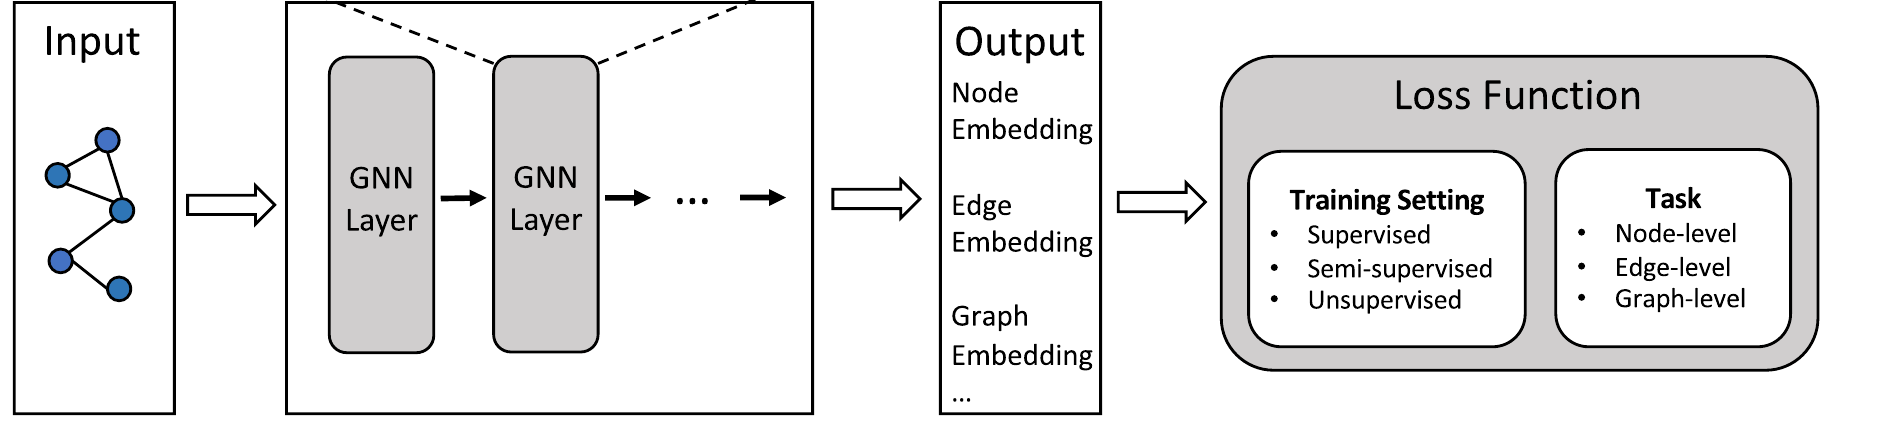
\includegraphics[width=\linewidth, keepaspectratio]{gnn/fig2_pipeline-v2.png}
  \vspace{0.3em}

  {\footnotesize\textit{Zhou et al. (2020), Fig. 2: pipeline tổng quát của GNN}}
\end{frame}


% ── Slide 4: Bức tranh Graph SSL ───────────────────────
\begin{frame}{Bức tranh Graph SSL: Contrastive vs.\ Generative}
  \vspace{0.3em}
  \centering
  \renewcommand{\arraystretch}{1.35}
  \small
  \begin{tabular}{p{2.1cm}p{5.2cm}p{5.2cm}}
    \toprule
    \textbf{Tiêu chí} & \textcolor{Theme_Color}{\textbf{Contrastive}} & \textcolor{orange!85!black}{\textbf{Generative}} \\
    \midrule
    \textbf{Ý tưởng} & Tạo 2 góc nhìn nhiễu, kéo cặp dương / đẩy cặp âm & Mã hóa đồ thị và tái tạo lại cấu trúc / đặc trưng \\
    \textbf{Đại diện} & DGI, GRACE, BGRL & GAE, MaskGAE, \textbf{GraphMAE} \\
    \textbf{Ưu điểm} & Học biểu diễn phân biệt tốt & Đơn giản, không cần augmentation phức tạp hay negative sampling \\
    \textbf{Nhược điểm} & Phụ thuộc phép tăng cường, tốn chi phí mẫu âm & Phụ thuộc mạnh vào ngữ cảnh láng giềng để tái tạo \\
    \bottomrule
  \end{tabular}
\end{frame}


% ── Slide 5: Graph Masked Autoencoder (GraphMAE) ──────
\begin{frame}{Generative methods}
  \centering
  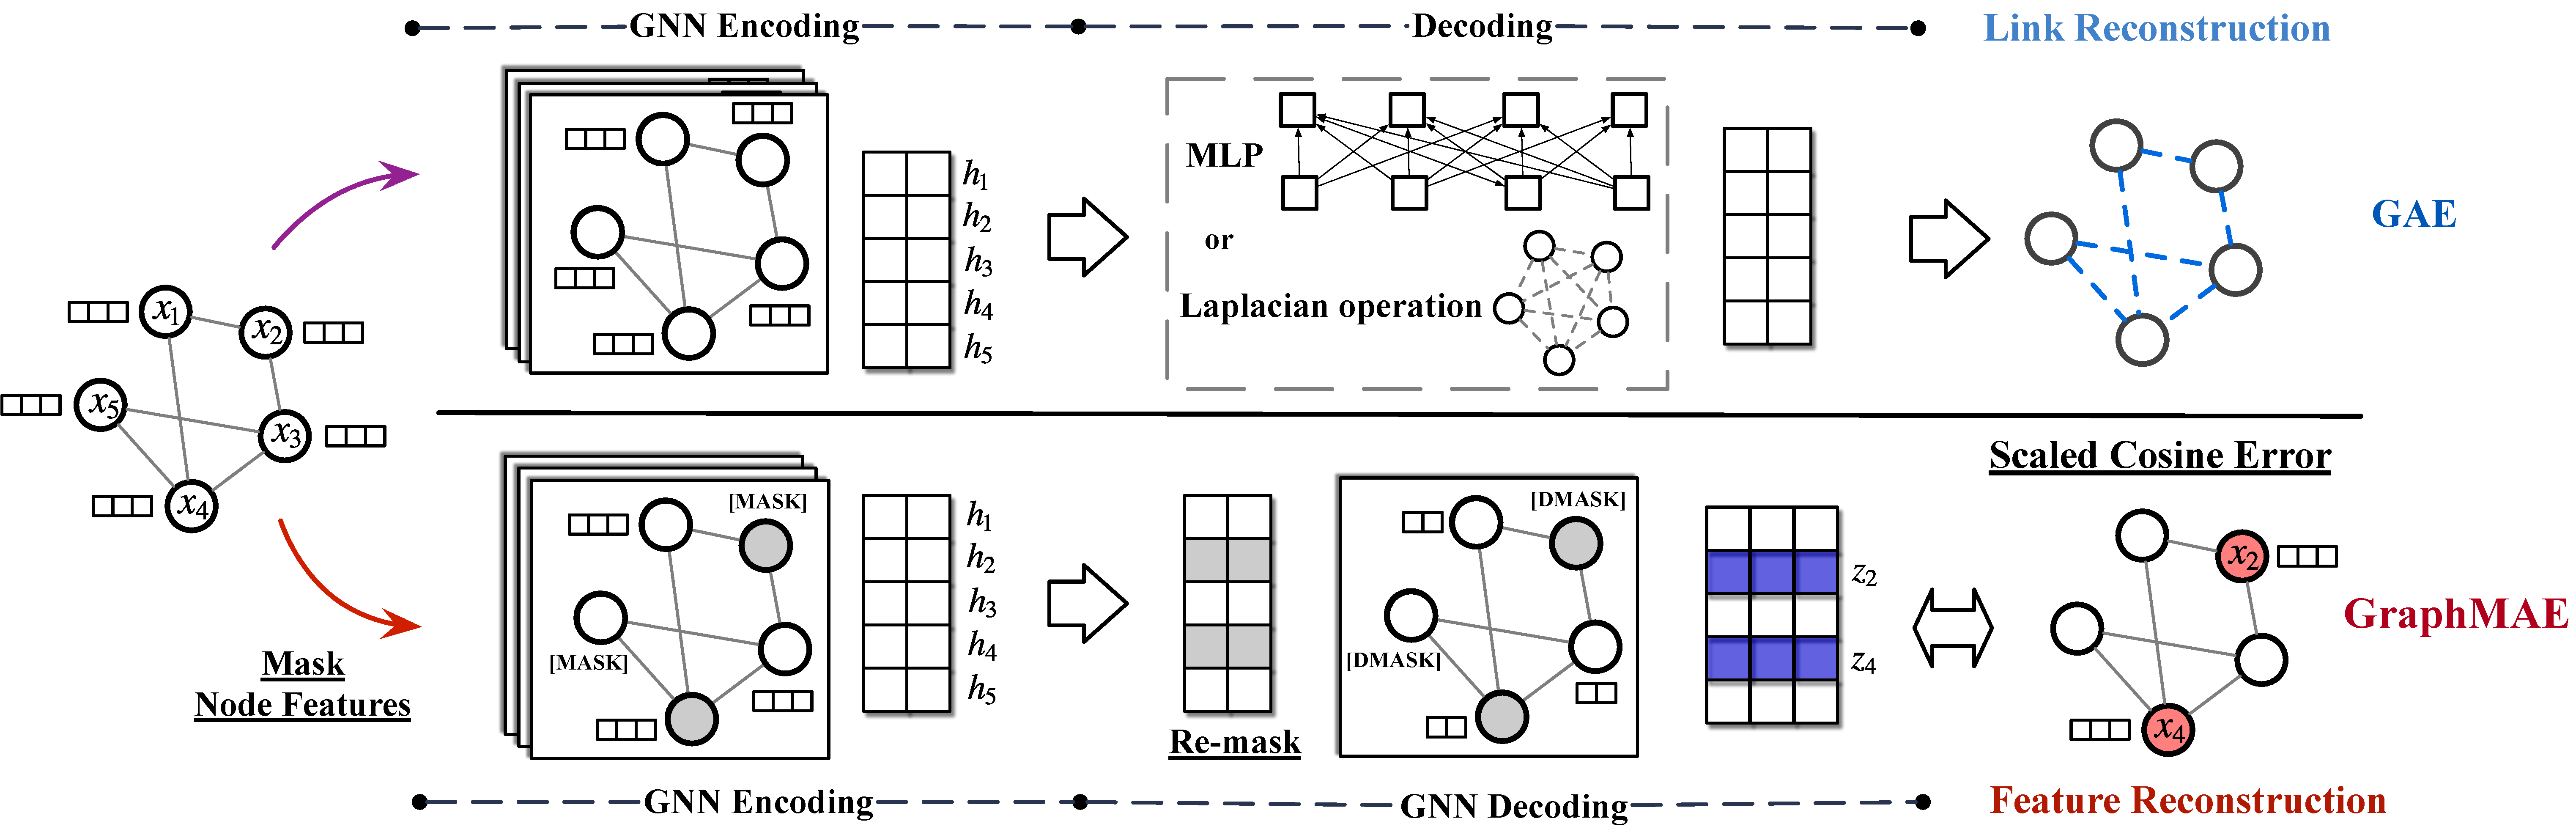
\includegraphics[width=0.84\linewidth, height=0.38\textheight, keepaspectratio]{arXiv-2205.10803v3/imgs/overview.pdf}
  \vspace{0.3em}

  \begin{columns}[T]
    \begin{column}{0.46\textwidth}
      \textcolor{Theme_Color}{\textbf{\small GAE — nhánh trên}}
      \vspace{0.3em}
      \begin{itemize}
        \setlength{\itemsep}{0.35em}
        \item Tái tạo \textbf{cạnh}: $A \rightarrow \hat{A}$
        \item Encoder GNN $\rightarrow$ decoder MLP
      \end{itemize}
    \end{column}

    \begin{column}{0.48\textwidth}
      \textcolor{orange!85!black}{\textbf{\small GraphMAE — nhánh dưới}}
      \vspace{0.3em}
      \begin{itemize}
        \setlength{\itemsep}{0.35em}
        \item Che đặc trưng nút: $X \rightarrow \hat{X}$
        \item Tái tạo \textbf{đặc trưng}, loss \textbf{SCE}
      \end{itemize}
    \end{column}
  \end{columns}
\end{frame}


% ── Slide 6: Đồng tính vs Dị tính — Định nghĩa ────────
\begin{frame}{Tính đồng tính vs.\ Tính dị tính: Định nghĩa}
  \vspace{0.2em}
  \begin{columns}[T]
    \begin{column}{0.48\textwidth}
      \textcolor{Theme_Color}{\textbf{\large Homophily (Đồng tính)}}
      \vspace{0.4em}
      \begin{itemize}
        \setlength{\itemsep}{0.4em}
        \item Phần lớn cạnh nối nút \textbf{cùng nhãn} ($y_i = y_j$)
        \item Tỉ lệ đồng tính $h$ \textbf{cao}
      \end{itemize}
      \vspace{0.5em}
      \centering
      \begin{tikzpicture}[
        scale=0.85,
        na/.style={circle, fill=Theme_Color!75, draw=Theme_Color, text=white, inner sep=0pt, minimum size=15pt, font=\scriptsize\bfseries},
        nb/.style={circle, fill=orange!80, draw=orange!90!black, text=white, inner sep=0pt, minimum size=15pt, font=\scriptsize\bfseries},
        ehomo/.style={thick, Theme_Color!80},
        ehet/.style={thick, orange!85!black, dashed}
      ]
        \node[na] (a1) at (0, 0.9) {$A$};
        \node[na] (a2) at (-1.1, 0) {$A$};
        \node[na] (a3) at (1.1, 0) {$A$};
        \node[na] (a4) at (0, -0.8) {$A$};
        \node[nb] (b1) at (2.2, 0.5) {$B$};
        \draw[ehomo] (a1) -- (a2);
        \draw[ehomo] (a1) -- (a3);
        \draw[ehomo] (a2) -- (a4);
        \draw[ehomo] (a3) -- (a4);
        \draw[ehomo] (a1) -- (a4);
        \draw[ehet]  (a3) -- (b1);
        \node[anchor=north, font=\scriptsize, text=black!70] at (0.5, -1.45) {$h = 5/6$};
      \end{tikzpicture}
    \end{column}

    \begin{column}{0.48\textwidth}
      \textcolor{orange!85!black}{\textbf{\large Heterophily (Dị tính)}}
      \vspace{0.4em}
      \begin{itemize}
        \setlength{\itemsep}{0.4em}
        \item Phần lớn cạnh nối nút \textbf{khác nhãn} ($y_i \neq y_j$)
        \item Tỉ lệ đồng tính $h$ \textbf{thấp}
      \end{itemize}
      \vspace{0.5em}
      \centering
      \begin{tikzpicture}[
        scale=0.85,
        na/.style={circle, fill=Theme_Color!75, draw=Theme_Color, text=white, inner sep=0pt, minimum size=15pt, font=\scriptsize\bfseries},
        nb/.style={circle, fill=orange!80, draw=orange!90!black, text=white, inner sep=0pt, minimum size=15pt, font=\scriptsize\bfseries},
        ehomo/.style={thick, Theme_Color!80},
        ehet/.style={thick, orange!85!black, dashed}
      ]
        \node[na] (a1) at (0, 0.9) {$A$};
        \node[nb] (b1) at (-1.1, 0) {$B$};
        \node[nb] (b2) at (1.1, 0) {$B$};
        \node[na] (a2) at (0, -0.8) {$A$};
        \node[na] (a3) at (2.2, 0.5) {$A$};
        \draw[ehet]  (a1) -- (b1);
        \draw[ehet]  (a1) -- (b2);
        \draw[ehet]  (b1) -- (a2);
        \draw[ehet]  (b2) -- (a2);
        \draw[ehet]  (b2) -- (a3);
        \draw[ehomo] (b1) -- (b2);
        \node[anchor=north, font=\scriptsize, text=black!70] at (0.5, -1.45) {$h = 1/6$};
      \end{tikzpicture}
    \end{column}
  \end{columns}

  \vspace{0.4em}
  \centering
  {\footnotesize Nét liền: cùng nhãn $\cdot$ Nét đứt: khác nhãn}\\[0.3em]
  $h = \dfrac{|\{(i,j) \in E : y_i = y_j\}|}{|E|}$
\end{frame}


% ── Slide 7: Vấn đề của GMAE trên đồ thị dị tính ─────
\begin{frame}{Vấn đề: Điểm yếu của GMAE trên đồ thị dị tính}
  \begin{columns}[T]
    \begin{column}{0.46\textwidth}
      \centering
      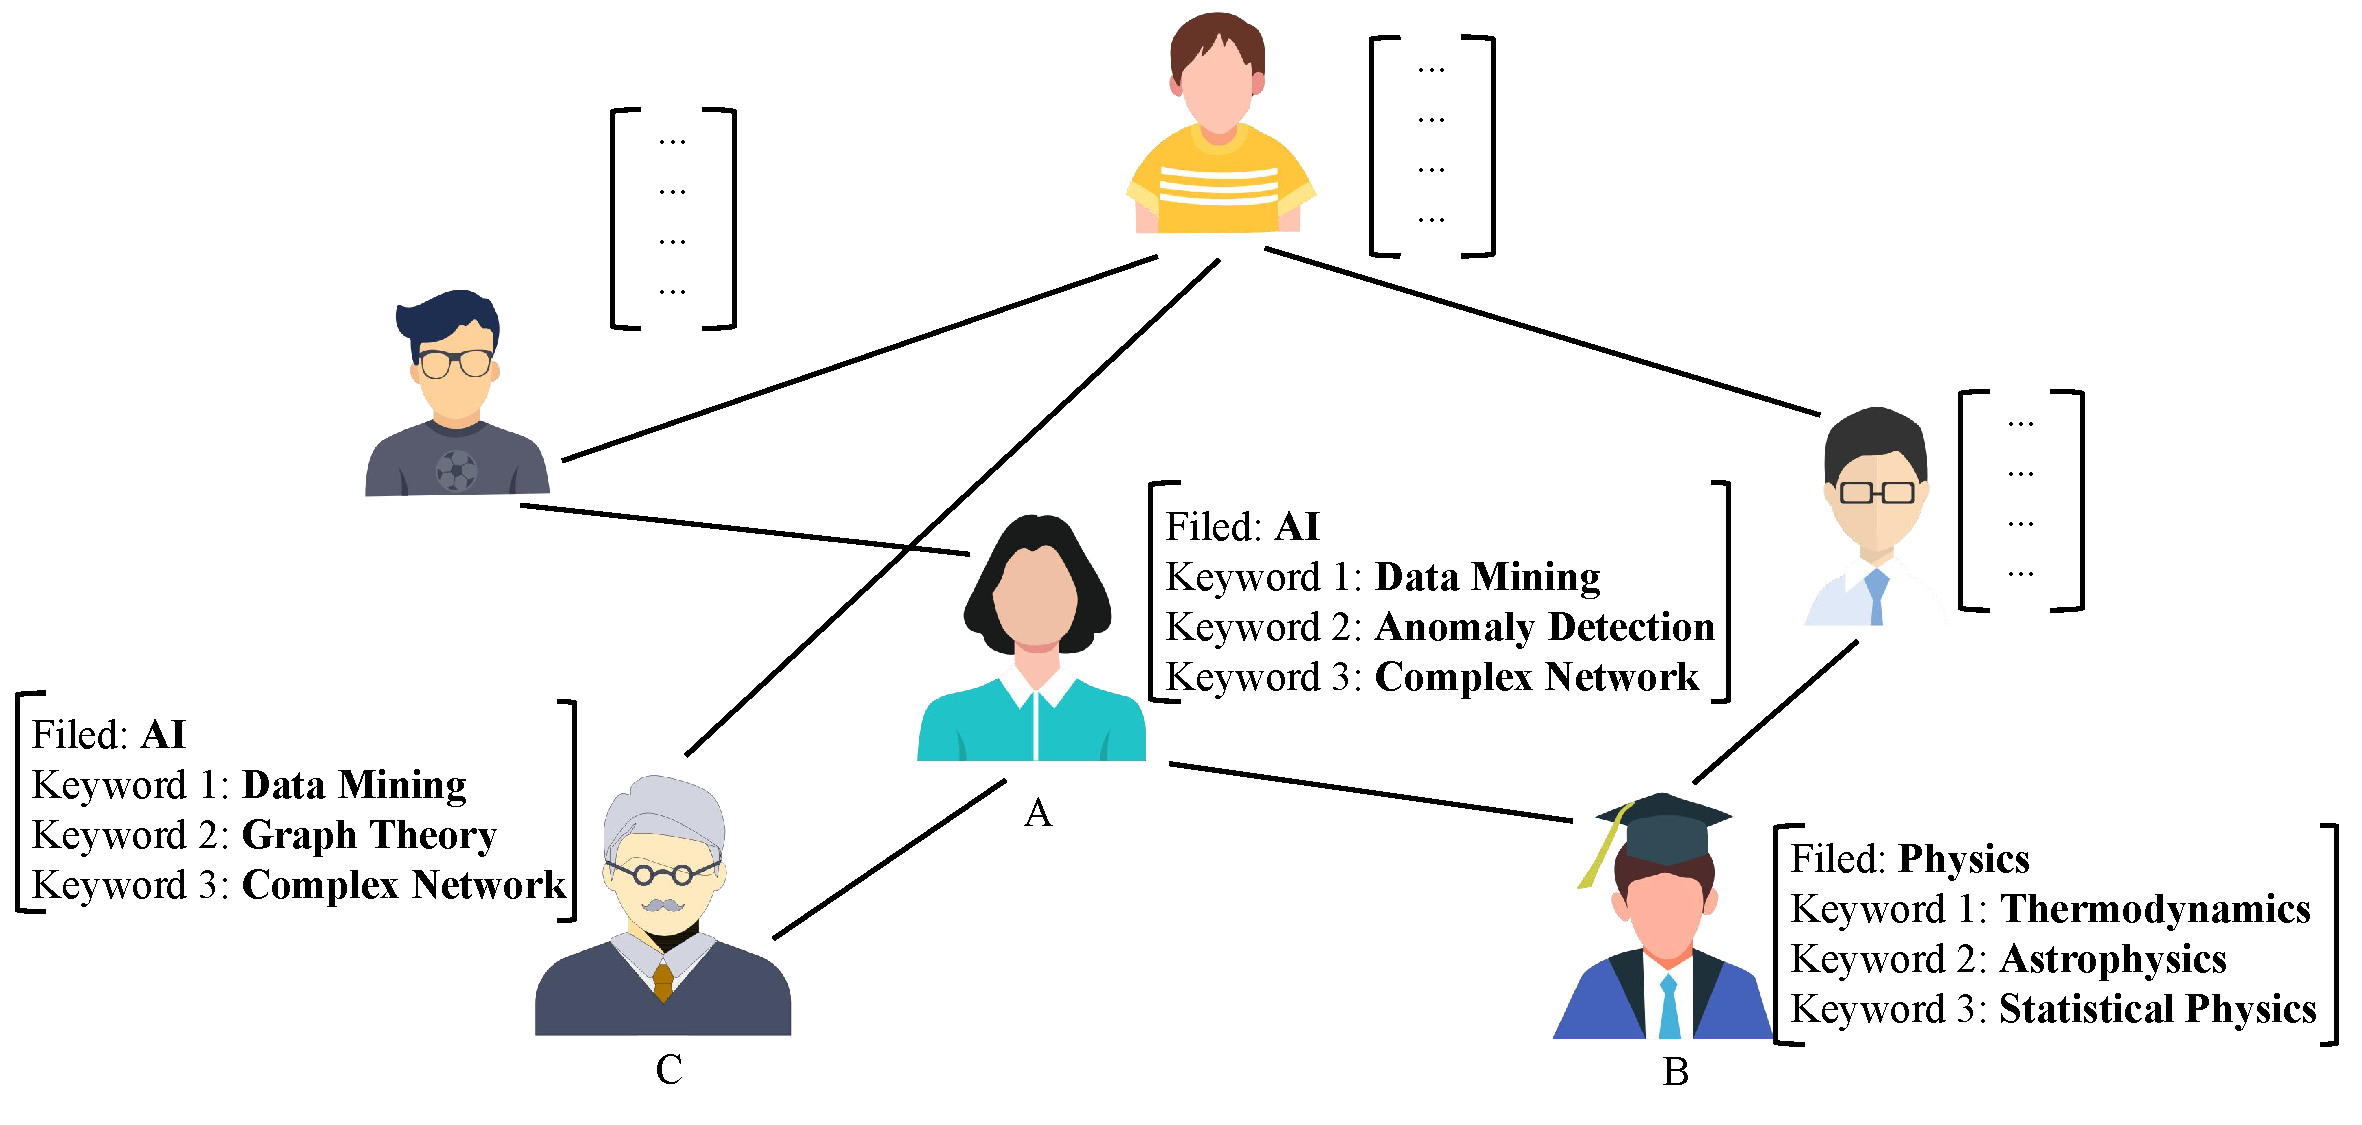
\includegraphics[width=\linewidth, height=0.45\textheight, keepaspectratio]{example.pdf}
      \vspace{0.4em} \\
      \small
      A (AI) $\leftrightarrow$ C (AI), B (Vật lý) \\
      Che A $\rightarrow$ B gây \textcolor{orange!85!black}{\textbf{nhiễu}}
    \end{column}

    \begin{column}{0.50\textwidth}
      \textcolor{orange!85!black}{\textbf{\large Điểm yếu cốt lõi}}
      \vspace{0.5em}
      \begin{itemize}
        \setlength{\itemsep}{0.6em}
        \item Thiên về \textbf{nhất quán (Consistency)}
        \item Thiếu \textbf{sai khác (Discrepancy)}
        \item Kéo nút khác lớp lại \textbf{gần nhau}
      \end{itemize}
    \end{column}
  \end{columns}
\end{frame}


% ── Slide 8: Thực nghiệm chứng minh vấn đề ────────────
\begin{frame}{Thực nghiệm chứng minh: Xóa nhòa sự khác biệt}
  \begin{columns}[T]
    \begin{column}{0.45\textwidth}
      \centering
      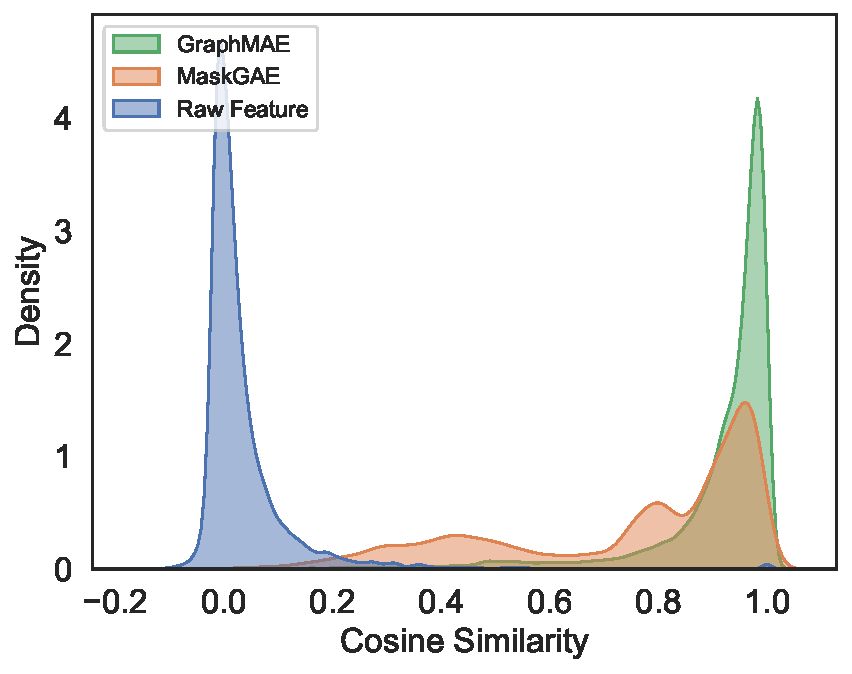
\includegraphics[width=\linewidth, height=0.55\textheight, keepaspectratio]{fig1.pdf}
      \vspace{0.2em} \\
      {\footnotesize\textit{Figure 2: Cosine similarity trên Squirrel}}
    \end{column}

    \begin{column}{0.52\textwidth}
      \textcolor{Theme_Color}{\textbf{\large Quan sát (Cặp nút khác lớp)}}
      \vspace{0.5em}
      \begin{itemize}
        \setlength{\itemsep}{0.6em}
        \item \textbf{Raw features:} $\approx 0$
        \item \textbf{GraphMAE / MaskGAE:} $\longrightarrow 1$
      \end{itemize}

      \vspace{0.8em}
      \textcolor{orange!85!black}{\textbf{\large Kết luận}}
      \vspace{0.4em}
      \begin{itemize}
        \item Tăng độ tương đồng nút khác lớp
        \item Giảm khả năng phân biệt biểu diễn
      \end{itemize}
    \end{column}
  \end{columns}
\end{frame}


% ── Slide 9: Động lực phát triển DGMAE ────────────────
\begin{frame}{Động lực phát triển: Thách thức \& Đóng góp của DGMAE}
  \vspace{0.3em}
  \textcolor{Theme_Color}{\textbf{\large Đóng góp (DGMAE)}}
  \vspace{0.6em}
  \begin{itemize}
    \setlength{\itemsep}{0.7em}
    \item \textbf{Tư duy mới:} Consistency $\rightarrow$ \textbf{Preserve Discrepancy}
    \item \textbf{Adaptive Selection:} Dùng attention chọn cạnh sai khác
    \item \textbf{Hiệu năng:} Tốt nhất \textbf{16/17} bộ dữ liệu
  \end{itemize}
\end{frame}


\section{Kiến trúc DGMAE}

% ── Slide 10: Kiến trúc tổng thể DGMAE ────────────────
\begin{frame}{Kiến trúc tổng thể DGMAE (Figure 3)}
  \centering
  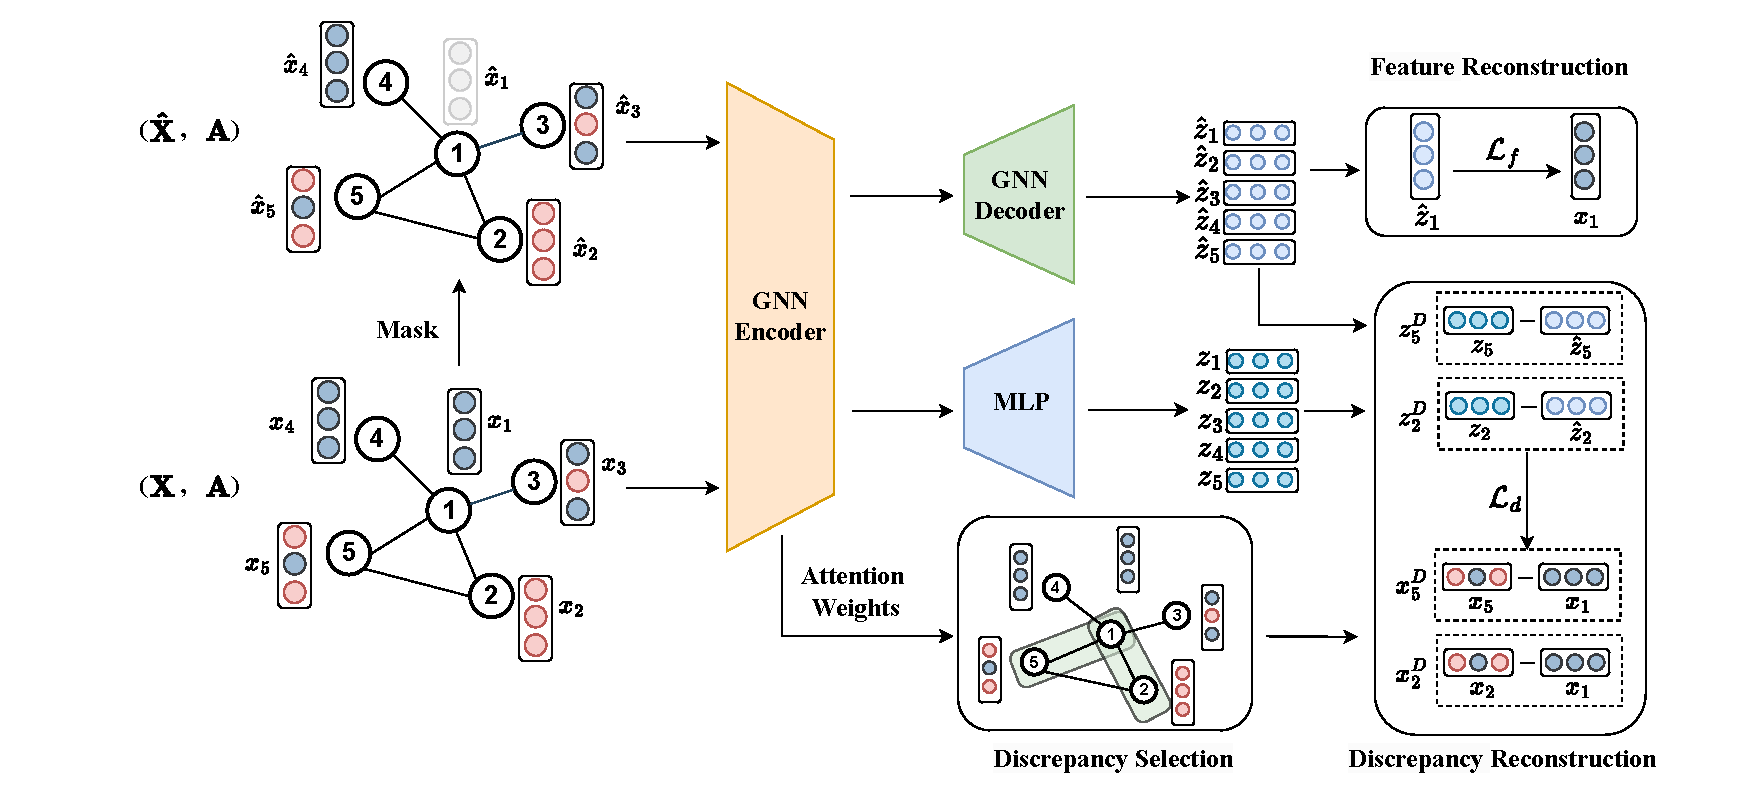
\includegraphics[width=0.92\linewidth, height=0.58\textheight, keepaspectratio]{model.pdf}
  \vspace{0.8em}

  {\large \textbf{2 Nhánh song song:} \quad Feature Recon. ($\mathcal{L}_f$) \quad $+$ \quad Discrepancy Recon. ($\mathcal{L}_d$)}

\end{frame}




% ══════════════════════════════════════════════════════
% PHẦN 2 — Phương pháp chính & Implement
% Người thuyết trình: B (TV4 — Trịnh Duy Hưng)  ~7.5 min
% ══════════════════════════════════════════════════════
% PHẦN 2 — Phương pháp DGMAE
% Nguồn: Zheng et al., KDD 2025, arXiv:2506.19343v2, §4.
% Mỗi frame tập trung vào một bước của phương pháp.

\section{Phương pháp DGMAE}

% 1. Định nghĩa mục tiêu
\begin{frame}{Sai khác gốc giữa nút và láng giềng}
  \begin{columns}[T,onlytextwidth]
    \begin{column}{0.48\textwidth}
      \centering
      \textcolor{Theme_Color}{\textbf{Dạng từng nút}}\\[1.2em]
      $\displaystyle x_i^D = x_i -
      \sum_{j\in\mathcal N(i)}\frac{x_j}{\sqrt{d_i d_j}}$\\[1.5em]
      {\small $x_i$: đặc trưng nút $i$;\\[0.4em]
      $\mathcal N(i)$: láng giềng của $i$;\\[0.4em]
      $d_i$: bậc của nút $i$.}
    \end{column}
    \begin{column}{0.48\textwidth}
      \centering
      \textcolor{Theme_Color}{\textbf{Dạng ma trận}}\\[1.2em]
      $\displaystyle X^D=L_{\mathrm{sym}}X$\\[0.6em]
      $\displaystyle L_{\mathrm{sym}}=I-D^{-1/2}AD^{-1/2}$\\[1.1em]
      {\small $X$: ma trận đặc trưng;\quad $A$: ma trận kề;\\[0.4em]
      $D$: ma trận bậc;\quad $I$: ma trận đơn vị;\\[0.4em]
      $L_{\mathrm{sym}}$: Laplacian chuẩn hóa.}
    \end{column}
  \end{columns}
  \vfill
  \centering
  \textbf{Đây là sai khác gốc; mục tiêu $\mathcal L_d$ sẽ được điều chỉnh sau khi chọn cạnh.}
  \vspace{0.5em}

  {\tiny Zheng et al., KDD 2025, Eq. (4)–(5)}
\end{frame}

% 2. Chọn cạnh bằng attention
\begin{frame}{Attention thấp làm cạnh dễ được chọn}
  \begin{columns}[T,onlytextwidth]
    \begin{column}{0.52\textwidth}
      \vspace{0.5em}
      $w_{ij}$: attention của cạnh $(i,j)$ từ GAT encoder.\\[1.0em]
      {\Large
      $\displaystyle p_{ij}=
      \min\!\bigl((1-w_{ij})p_c,\,p_\tau\bigr)$
      }\\[0.9em]
      $m_{ij}\sim\mathrm{Bernoulli}(p_{ij})$\\[1.0em]
      \small $p_{ij}$: xác suất chọn cạnh;\quad $m_{ij}=1$: cạnh được chọn.\\[0.35em]
      $p_c$: mức lấy mẫu;\quad $p_\tau$: giới hạn xác suất.\\[0.35em]
      % Bernoulli: phép lấy mẫu nhị phân.
    \end{column}
    \begin{column}{0.45\textwidth}
      \centering
      \begin{tikzpicture}[scale=1.02,
        every node/.style={font=\small},
        point/.style={circle,draw=Theme_Color,fill=Theme_Color!12,minimum size=8mm}]
        \node[point] (i) at (0,0) {$i$};
        \node[point] (a) at (2.2,1.2) {$j_1$};
        \node[point] (b) at (2.2,-1.2) {$j_2$};
        \draw[very thick,Theme_Color] (i) -- node[above,sloped,font=\scriptsize] {$w$ cao} (a);
        \draw[very thick,orange!90!black,dashed] (i) -- node[below,sloped,font=\scriptsize] {$w$ thấp} (b);
      \end{tikzpicture}\\[0.7em]
      \small\textcolor{orange!90!black}{\textbf{Cạnh nét đứt:}} có $p_{ij}$ cao hơn.
    \end{column}
  \end{columns}
  \vfill
  \centering
  {\tiny Zheng et al., KDD 2025, Eq. (6)–(8)}
\end{frame}

% 3. Mục tiêu sau chọn cạnh
\begin{frame}{Đích sai khác chỉ dùng cạnh được chọn}
  \centering
  \vspace{0.8em}
  {\Large
  $\displaystyle x_i^D=
  \sum_{j\in\mathcal N(i)}
  \frac{m_{ij}}{\sqrt{d_i d_j}}(x_i-x_j)$
  }
  \vspace{1.2em}

  \begin{columns}[T,onlytextwidth]
    \begin{column}{0.48\textwidth}
      \centering
      \textcolor{Theme_Color}{\Large $m_{ij}=0$}\\[0.45em]
      Cạnh không đóng góp vào đích $x_i^D$.
    \end{column}
    \begin{column}{0.48\textwidth}
      \centering
      \textcolor{orange!90!black}{\Large $m_{ij}=1$}\\[0.45em]
      Giữ chênh lệch $x_i-x_j$ của cặp nút.
    \end{column}
  \end{columns}
  \vfill
  \textbf{$x_i^D$ tổng hợp chênh lệch đặc trưng giữa nút $i$ và các láng giềng được chọn.}
  \vspace{0.5em}

  {\tiny Zheng et al., KDD 2025, Eq. (9)}
\end{frame}

% 4. Giới thiệu hai nhánh
\begin{frame}{Hai nhánh huấn luyện DGMAE}
  \centering
  % \vspace{0.3em}
  % Cùng ma trận kề $A$ và cùng encoder $f_E$;
  % hai nhánh khác nhau ở đặc trưng đầu vào.
  \vspace{1.2em}

  \begin{columns}[T,onlytextwidth]
    \begin{column}{0.48\textwidth}
      \centering
      \textcolor{Theme_Color}{\Large Nhánh đồ thị bị che}\\[0.8em]
      $\hat X\xrightarrow{f_E}\hat H\xrightarrow{f_D}\hat Z$\\[1.0em]
      \textbf{$\mathcal L_f$:} khôi phục đặc trưng\\
      trên các nút bị che $\hat V$.
    \end{column}
    \begin{column}{0.48\textwidth}
      \centering
      \textcolor{orange!90!black}{\Large Nhánh đồ thị không che}\\[0.8em]
      $X\xrightarrow{f_E}H\xrightarrow{\mathrm{MLP}}Z$\\[1.0em]
      \textbf{$\mathcal L_d$:} giữ sai khác\\
      trên các nút không bị che $V\setminus\hat V$.
    \end{column}
  \end{columns}
  \vspace{1.4em}

  {\large $z_i^D=z_i-\hat z_i$}\\[0.5em]
  \textbf{$\mathcal L_d$ cần cả $Z$ và $\hat Z$; hai nhánh được huấn luyện chung.}
  \vfill
  {\tiny Zheng et al., KDD 2025, §4.2–4.4}
\end{frame}

% 5. Nhánh đồ thị bị che và loss tái tạo
\begin{frame}{Nhánh đồ thị bị che: tái tạo đặc trưng}
  \begin{columns}[T,onlytextwidth]
    \begin{column}{0.47\textwidth}
      \centering
      \textcolor{Theme_Color}{\bfseries Đồ thị bị che}\\[1.0em]
      $\displaystyle \hat x_i=0\quad(i\in\hat V)$\\[1.1em]
      $\hat X\xrightarrow{f_E}\hat H\xrightarrow{f_D}\hat Z$\\[1.1em]
      {Decoder $f_D$ dùng ngữ cảnh láng giềng
      để tái tạo đặc trưng của nút bị che.}\\[1.0em]
      {\small $x_i$ gốc được giữ làm mục tiêu,
      không đưa vào lượt xử lý này.}
    \end{column}
    \begin{column}{0.50\textwidth}
      \centering
      \textcolor{Theme_Color}{\bfseries Loss tái tạo $\mathcal L_f$}\\[1.0em]
      {\small $\displaystyle
        % Eq. (3) prints z_i, but Eq. (2), the prose, and author code
        % compare decoder output \hat z_i with original x_i.
        \mathcal L_f=
        \frac{1}{|\hat V|}
        \sum_{i\in\hat V}
        \bigl(1-\cos(\hat z_i,x_i)\bigr)^{\gamma_1}
      $}\\[1.1em]
      \textbf{So sánh $\hat z_i$ với $x_i$}\\
      trên \textbf{nút bị che}.\\[1.0em]
      {\small $\cos$: độ tương đồng cosine;\\[0.4em]
      $\gamma_1>1$: số mũ điều chỉnh loss.}
    \end{column}
  \end{columns}
  \vfill
  \centering
  {\tiny Zheng et al., KDD 2025, Eq. (1)–(3)}
\end{frame}

% 6. Nhánh đồ thị đầy đủ và loss sai khác
\begin{frame}{Nhánh đồ thị không che: giữ sai khác}
  \begin{columns}[T,onlytextwidth]
    \begin{column}{0.47\textwidth}
      \centering
      \textcolor{orange!90!black}{\bfseries Đồ thị không che}\\[1.0em]
      $X\xrightarrow{f_E}H\xrightarrow{\mathrm{MLP}}Z$\\[1.0em]
      {Projector MLP đưa $H$ về cùng không gian
      đặc trưng với $\hat Z$.}\\[1.1em]
      {\large $z_i^D=z_i-\hat z_i$}\\[0.7em]
      {\small $\hat z_i$ đến từ nhánh có che;
      $x_i^D$ là mục tiêu tính từ các cạnh được chọn.}
    \end{column}
    \begin{column}{0.50\textwidth}
      \centering
      \textcolor{orange!90!black}{\bfseries Loss sai khác $\mathcal L_d$}\\[1.0em]
      {\small $\displaystyle
        \mathcal L_d=
        % Eq. (12) in the paper prints |\hat V|, but its sum and prose use
        % unmasked nodes; the authors' code averages over keep_nodes.
        \frac{1}{|V\setminus\hat V|}
        \sum_{i\in V\setminus\hat V}
        \bigl(1-\cos(z_i^D,x_i^D)\bigr)^{\gamma_2}
      $}\\[1.1em]
      \textbf{So sánh $z_i^D$ với $x_i^D$}\\
      trên \textbf{nút không bị che}.\\[1.0em]
      {\small $\cos$: độ tương đồng cosine;\\[0.4em]
      $\gamma_2>1$: số mũ điều chỉnh loss.}
    \end{column}
  \end{columns}
  \vfill
  \centering
  {\tiny Zheng et al., KDD 2025, Eq. (10)–(12); tập nút theo phần giải thích sau Eq. (12)}
\end{frame}

% 7. Mục tiêu chung
\begin{frame}{Huấn luyện DGMAE: loss và một epoch}
  \begin{columns}[T,onlytextwidth]
    \begin{column}{0.48\textwidth}
      \centering
      \textcolor{Theme_Color}{\bfseries Hàm mất mát tổng}\\[1.0em]
      {\large $\displaystyle
        \mathcal L=(1-\lambda)\mathcal L_f+\lambda\mathcal L_d
      $}\\[1.3em]

      \textcolor{Theme_Color}{\Large $\mathcal L_f$}\\[0.3em]
      Khôi phục đặc trưng $x_i$\\
      trên \textbf{nút bị che}\\[1.1em]

      \textcolor{orange!90!black}{\Large $\mathcal L_d$}\\[0.3em]
      Giữ sai khác $x_i^D$\\
      trên \textbf{nút không bị che}\\[1.2em]

      {\small $\lambda$ điều chỉnh trọng số của hai loss.}
    \end{column}
    \begin{column}{0.49\textwidth}
      \centering
      \textcolor{Theme_Color}{\bfseries Một epoch huấn luyện}\\[0.7em]
      \begin{tikzpicture}[
        flowbox/.style={draw=Theme_Color, fill=Theme_Color!8,
          rounded corners=2pt, minimum width=5.5cm, minimum height=0.9cm,
          align=center, font=\small},
        flow/.style={->, thick, Theme_Color}
      ]
        \node[flowbox] (mask) at (0,0) {1. Che đặc trưng nút\\$X\rightarrow\hat X$};
        \node[flowbox] (encode) at (0,-1.28) {2. Hai lượt xử lý đồ thị\\$\hat X\rightarrow\hat Z,\quad X\rightarrow Z$};
        \node[flowbox] (diff) at (0,-2.56) {3. Chọn cạnh và tính sai khác\\$x_i^D,\quad z_i^D$};
        \node[flowbox] (loss) at (0,-3.84) {4. Tính loss và cập nhật\\$\mathcal L_f,\mathcal L_d\rightarrow\mathcal L$};
        \draw[flow] (mask) -- (encode);
        \draw[flow] (encode) -- (diff);
        \draw[flow] (diff) -- (loss);
      \end{tikzpicture}
    \end{column}
  \end{columns}
  \vfill
  \centering
  {\tiny Zheng et al., KDD 2025, §4.2–4.4, Eq. (13)}
\end{frame}

\section{Implement của nhóm}

\begin{frame}{Implement: cấu trúc code}
  % TODO: Cấu trúc repo, framework, phần cứng
\end{frame}

\begin{frame}{Implement: khó khăn \& đối chiếu}
  % TODO: Khó khăn gặp phải, so sánh với code tác giả
\end{frame}


% ══════════════════════════════════════════════════════
% PHẦN 3 — Thực nghiệm, Phân tích, Kết luận
% Người thuyết trình: C (TV5 — Lương Huỳnh Gia Bảo)  ~9.5 min
% ══════════════════════════════════════════════════════
% ══════════════════════════════════════════════════════
% PHẦN 3 — Thực nghiệm, Phân tích, Kết luận   (SƯỜN — chờ kết quả chạy chính thức trên Kaggle)
% Người thuyết trình: C (TV5 — Lương Huỳnh Gia Bảo)
% Thời lượng: ~10 phút (10 slide nội dung, ~1 phút/slide)
% ══════════════════════════════════════════════════════
%
% Mạch trình bày: kết quả chính (dị tính → đồng tính/đồ thị → tái lập) → phân tích → Key findings → kết luận.
%
% Quy ước: nhóm chỉ chạy lại DGMAE (code C:/DGMAE/DGMAE-REIMPL, chạy trên Kaggle, 10 seed 0–9);
%   số của mọi phương pháp khác lấy từ paper. Ô của nhóm tô đỏ (\nh), dòng DGMAE của paper in đậm (\dg).
% Trình bày: 1 cột; chỉ chia 2 cột khi hai bên cân nhau (cùng rộng, cùng loại nội dung).
%   Mỗi slide: 1 bảng/hình + 1 dòng kết luận (\ketluan) dạng "Paper: … · Nhóm: …"; chi tiết để ở "Lời thoại".
% [ĐIỀN] = chờ kết quả chính thức · [KIỂM TRA] = cần đối chiếu lại với paper.
%
% Slide nào lấy số từ nhóm chạy Kaggle nào (GROUP trong kaggle/run_on_kaggle.ipynb):
%   Phân loại dị tính, Phân cụm  ← main_small, main_mid, main_roman
%   Đồng tính & đồ thị           ← main_small, main_mid (Cora/Citeseer/Pubmed) · graph (Table 9)
%   Tái lập (biểu đồ)            ← vẽ lại: python scripts/plot_paper_vs_team.py
%   Ablation                     ← ablation (+ bản đầy đủ từ main_small)
%   Độ nhạy λ                    ← lambda (+ λ theo Table 8 từ main_small)

% ── Macro dùng riêng trong phần 3 ──
\newcommand{\dg}[1]{\textbf{#1}}                                  % ô của dòng DGMAE (paper): đen đậm
\newcommand{\nh}[1]{\textcolor{Theme_Color}{#1}}                  % ô của nhóm chạy lại: đỏ (khớp biểu đồ)
\newcommand{\pmstd}[1]{{\tiny$\pm$#1}}                            % std nhỏ
\newcommand{\dien}{\nh{[ĐIỀN]}}                                   % ô kết quả nhóm chưa có
\newcommand{\ketluan}[1]{%
  \vfill
  \begin{center}
    \colorbox{RiverLight}{\parbox{0.94\textwidth}{\centering\small\vspace{0.35em}#1\vspace{0.35em}}}
  \end{center}}
\newcommand{\hinhcho}[3]{%                                         % khung giữ chỗ cho hình chưa có: {rộng}{cao}{nội dung}
  \tikz\node[draw=gray!60, dashed, rounded corners, minimum width=#1, minimum height=#2,
             align=center, text=gray, font=\small]{#3};}

\section{Experiments}

% ── Slide: Thiết lập thực nghiệm ─────────────────────
\begin{frame}{Experimental Setup}
  \centering
  \textbf{Self-supervised} pre-training $\rightarrow$ frozen encoder $\rightarrow$ evaluate embeddings (Sec.~5.3)\\[1em]
  \renewcommand{\arraystretch}{1.4}
  \begin{tabular}{l l l}
    \toprule
    \textbf{Task} & \textbf{Datasets} & \textbf{Evaluation} \\
    \midrule
    Node classification  & 7 heterophilic, 3 homophilic graphs & Logistic regression \\
    Node clustering      & 6 heterophilic graphs               & K-means \\
    Graph classification & MUTAG, PROTEINS, IMDB-M, COLLAB     & SVM (10-fold CV) \\
    \bottomrule
  \end{tabular}
  \ketluan{We re-run \textbf{DGMAE only} (10 seeds, hyper-parameters from Table~8, Kaggle GPU) ·
    baselines: \textbf{numbers reported in the paper}}
  % Lời thoại:
  % - Dị tính: Texas, Cornell, Wisconsin, Chameleon, Squirrel, Actor, Roman-empire. Đồng tính: Cora, Citeseer, Pubmed.
  % - Giao thức chuẩn của học biểu diễn tự giám sát: encoder học không nhãn rồi đóng băng; chất lượng embedding
  %   đo bằng một mô hình đơn giản đặt lên trên (linear probing). Báo cáo mean ± std của 10 lần chạy.
  % - Split: Planetoid public; dị tính 10 split Geom-GCN (48/32/20); Roman 10 split (50/25/25).
  % - Code cài lại từ đầu (PyTorch, GAT tự viết), không dùng code tác giả. GPU Kaggle [ĐIỀN: P100/T4] (paper: TITAN RTX 24 GB).
  % - Paper không nêu hidden size, số head, số epoch, tiền xử lý, cấu hình linear probe → nhóm lấy theo config tác giả;
  %   linear probe: Adam, lr 0.01, wd 1e-4, 300 epoch, chọn epoch theo tập val.
  % - Không chạy: Crocodile, Amazon, Coauthor, WikiCS, Flickr và 5 đồ thị lớn ở Table 11 (thời gian, GPU).
\end{frame}

% ── Slide: Phân loại node — dị tính (Table 1) ────────
\begin{frame}{Node Classification on Heterophilic Graphs}
  \centering
  \resizebox{0.96\textwidth}{!}{%
    \begin{tabular}{ll ccccccc}
      \toprule
      & \textbf{Method} & \textbf{Texas} & \textbf{Cornell} & \textbf{Wisconsin} & \textbf{Chameleon} & \textbf{Squirrel} & \textbf{Actor} & \textbf{Roman} \\
      \midrule
      \multirow{3}{*}{Contrastive}
        & GREET    & \underline{82.70} & 73.78 & \underline{82.94} & 63.64 & 42.29 & \underline{36.55} & 50.69 \\
        & SP-GCL   & 80.36 & \underline{78.33} & 78.26 & 65.28 & 52.10 & 28.94 & 70.88 \\
        & GraphACL & 71.08 & 59.33 & 69.22 & 69.12 & 54.05 & 30.03 & \underline{74.91} \\
      \midrule
      \multirow{3}{*}{Generative}
        & NWR-GAE  & 69.62 & 58.64 & 68.23 & 72.04 & \underline{64.81} & 30.17 & 46.35 \\
        & AUG-MAE  & 72.97 & 65.14 & 76.47 & \underline{72.19} & 53.23 & 26.36 & 51.13 \\
        & GraphMAE & 55.14 & 51.62 & 55.69 & 68.67 & 44.91 & 25.61 & 46.73 \\
      \midrule
      & \dg{DGMAE (paper)}
        & \dg{88.11}\pmstd{5.16} & \dg{78.65}\pmstd{4.59} & \dg{88.43}\pmstd{3.56} & \dg{75.50}\pmstd{1.17}
        & \dg{72.47}\pmstd{1.77} & \dg{36.61}\pmstd{0.74} & \dg{76.62}\pmstd{0.41} \\
      & \nh{DGMAE (repro.)} & \dien & \dien & \dien & \dien & \dien & \dien & \dien \\
      \bottomrule
    \end{tabular}%
  }\\[0.3em]
  {\scriptsize Accuracy (\%). Baselines from Table~1 of the paper; \underline{underline}: runner-up.}
  \ketluan{Paper: DGMAE \textbf{ranks 1st on all 7 datasets} · Reproduced: [ĐIỀN: hạng 1 ở bao nhiêu dataset?]}
  % Lời thoại:
  % - Bảng chỉ giữ các phương pháp đứng thứ hai ở ít nhất một dataset (và GraphMAE để so sánh).
  %   Std của các phương pháp khác xem Table 1 của paper.
  % - Paper kết luận: DGMAE vượt cả các phương pháp contrastive thiết kế riêng cho đồ thị dị tính
  %   → L_d giải quyết được vấn đề đồng nhất hóa của GMAE.
  % - Nhóm: [ĐIỀN: so số của nhóm với các baseline của paper — thua phương pháp nào, ở dataset nào].
\end{frame}

% ── Slide: Phân cụm node (Table 3) ───────────────────
\begin{frame}{Node Clustering on Heterophilic Graphs}
  \centering
  \resizebox{0.96\textwidth}{!}{%
    \begin{tabular}{ll cccccc}
      \toprule
      & \textbf{Method} & \textbf{Texas} & \textbf{Cornell} & \textbf{Wisconsin} & \textbf{Chameleon} & \textbf{Squirrel} & \textbf{Roman} \\
      \midrule
      \multirow{4}{*}{ACC}
        & GREET    & 52.40 & 48.96 & 56.65 & 34.44 & 25.64 & 31.43 \\
        & GraphMAE & 46.28 & 46.12 & 52.67 & 37.02 & 27.61 & 15.38 \\
        & \dg{DGMAE (paper)} & \dg{66.83}\pmstd{6.19} & \dg{57.16}\pmstd{5.99} & \dg{68.69}\pmstd{4.52} & \dg{39.96}\pmstd{1.74} & \dg{30.83}\pmstd{0.71} & \dg{36.25}\pmstd{0.86} \\
        & \nh{DGMAE (repro.)}  & \dien & \dien & \dien & \dien & \dien & \dien \\
      \midrule
      \multirow{4}{*}{NMI}
        & GREET    & 37.19 & 28.19 & 22.57 & 14.99 &  3.22 & 37.00 \\
        & GraphMAE &  6.06 & 12.07 & 18.54 & 19.47 &  4.58 &  9.33 \\
        & \dg{DGMAE (paper)} & \dg{37.41}\pmstd{7.20} & \dg{34.41}\pmstd{7.88} & \dg{44.19}\pmstd{2.19} & \dg{22.39}\pmstd{0.43} & \dg{8.00}\pmstd{0.73} & \dg{37.57}\pmstd{0.53} \\
        & \nh{DGMAE (repro.)}  & \dien & \dien & \dien & \dien & \dien & \dien \\
      \bottomrule
    \end{tabular}%
  }\\[0.3em]
  {\scriptsize K-means on embeddings (\%). GREET, GraphMAE from Table~3 of the paper; ARI and F1 show the same trend.}
  \ketluan{Paper: DGMAE \textbf{ranks 1st in all 24 cells} (6 datasets $\times$ 4 metrics) · Reproduced: [ĐIỀN]}
  % Lời thoại:
  % - Phân cụm khó hơn phân loại vì không dùng nhãn nào. GraphMAE gần như "mù" trên Texas (NMI 6, ARI ~1).
  % - Paper: cách biệt lớn nhất ở ARI (Texas +18.0, Wisconsin +19.2 so với GREET).
  % - Hạng 2 ở Texas ACC là NWR-GAE (55.03); ở Squirrel F1 là MaskGAE (23.27); các ô còn lại là GREET hoặc GraphMAE.
  % - Nhóm (ARI, F1 — không đưa lên slide): [ĐIỀN].
\end{frame}

% ── Slide: Đồng tính (Table 2) & phân loại đồ thị (Table 9) — 2 cột cân nhau: mỗi bên 4 baseline + 2 dòng DGMAE ──
\begin{frame}{Homophilic Graphs \& Graph Classification}
  \begin{columns}[t]
    \begin{column}{0.48\textwidth}
      \centering
      {\small\textbf{Node classification — Table~2}}\\[0.4em]
      {\scriptsize\setlength{\tabcolsep}{3pt}
      \begin{tabular}{l ccc}
        \toprule
        \textbf{Method} & \textbf{Cora} & \textbf{Citeseer} & \textbf{Pubmed} \\
        \midrule
        GraphACL & 84.20 & \underline{73.63} & 82.02 \\
        NWR-GAE  & 83.62 & 71.45 & \underline{83.44} \\
        Bandana  & \underline{84.62} & 73.60 & \textbf{83.53} \\
        GraphMAE & 84.20 & 73.40 & 81.10 \\
        \midrule
        \dg{DGMAE (paper)} & \dg{84.93}\pmstd{0.51} & \dg{73.82}\pmstd{0.64} & 81.10\pmstd{0.42} \\
        \nh{DGMAE (repro.)}  & \dien & \dien & \dien \\
        \bottomrule
      \end{tabular}}
    \end{column}
    \begin{column}{0.48\textwidth}
      \centering
      {\small\textbf{Graph classification — Table~9}}\\[0.4em]
      {\scriptsize\setlength{\tabcolsep}{3pt}
      \begin{tabular}{l cccc}
        \toprule
        \textbf{Method} & \textbf{MUTAG} & \textbf{PROTEINS} & \textbf{IMDB-M} & \textbf{COLLAB} \\
        \midrule
        Infograph & \underline{89.01} & 74.44 & 49.69 & 70.65 \\
        S2GAE     & 88.26 & \underline{76.37} & 51.79 & \underline{81.02} \\
        AUG-MAE   & 88.28 & 75.83 & \underline{51.80} & 80.48 \\
        GraphMAE  & 88.19 & 75.30 & 51.63 & 80.32 \\
        \midrule
        \dg{DGMAE (paper)} & \dg{89.06}\pmstd{0.64} & \dg{76.51}\pmstd{0.52} & \dg{51.95}\pmstd{0.30} & \dg{81.15}\pmstd{0.30} \\
        \nh{DGMAE (repro.)}  & \dien & \dien & \dien & \dien \\
        \bottomrule
      \end{tabular}}
    \end{column}
  \end{columns}
  \vspace{0.5em}
  \centering{\scriptsize Accuracy (\%). Baselines from the paper; \underline{underline}: runner-up.}
  \ketluan{Paper: 1st on Cora, Citeseer and all 4 graph datasets $\Rightarrow$ $\mathcal{L}_d$ \textbf{does not hurt} · Reproduced: [ĐIỀN]}
  % Lời thoại:
  % - DGMAE được thiết kế cho đồ thị dị tính; ở đây paper chỉ cần chứng minh "không làm hại".
  % - Table 2 trên slide chỉ giữ phương pháp hạng 2 / tốt nhất ở ít nhất một dataset và GraphMAE
  %   (GREET 83.82/73.22/80.20, AUG-MAE 84.30/73.20/81.12 — xem Table 2 của paper).
  % - Pubmed: DGMAE của paper bằng GraphMAE (81.10), không đứng đầu (Bandana 83.53 tốt nhất — in đậm).
  % - Phân loại đồ thị: encoder GIN; L_d dùng L_sym X (Eq. 5). Table 8 không có siêu tham số cho tác vụ này → theo config tác giả.
  % - Nhóm: [ĐIỀN].
\end{frame}

% ── Slide: Tái lập: nhóm vs. paper ───────────────────
\begin{frame}{Reproducibility: Reproduced vs.\ Paper}
  \centering
  % Khi có kết quả: chạy  python scripts/plot_paper_vs_team.py  (trong DGMAE-REIMPL), rồi thay khung dưới bằng:
  %   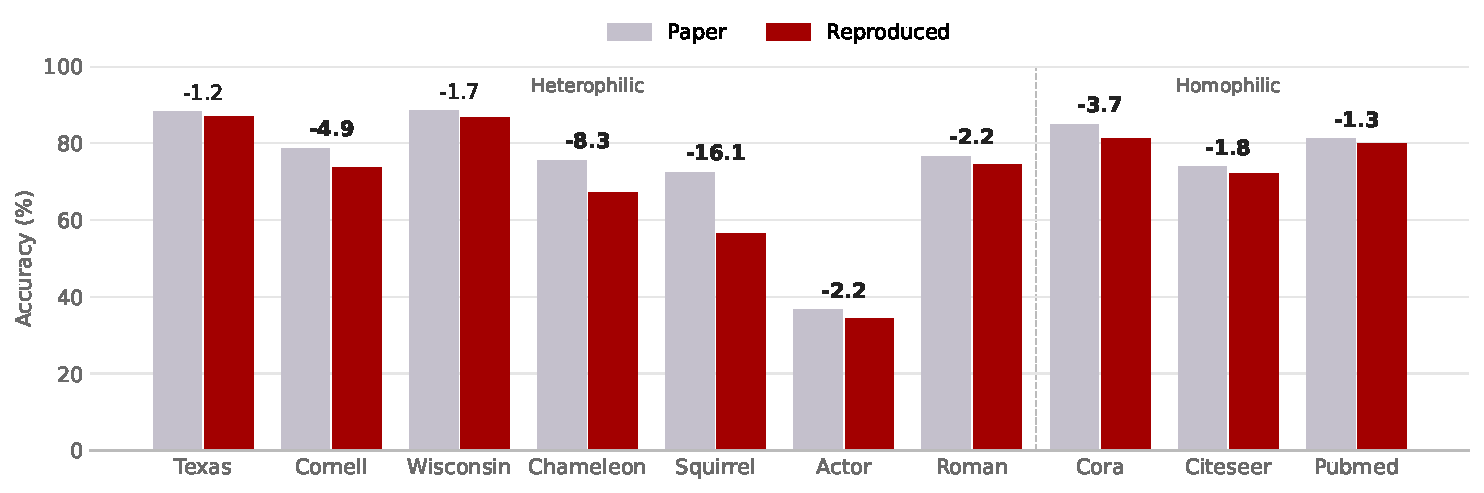
\includegraphics[width=\textwidth]{paper_vs_nhom.pdf}
  \hinhcho{0.95\textwidth}{0.52\textheight}{[ĐIỀN] Bar chart: DGMAE accuracy, paper vs.\ reproduced, 10 datasets\\
    (label: reproduced $-$ paper; bold if outside 1 std)}\\[0.1em]
  {\scriptsize DGMAE node classification accuracy. Labels: reproduced $-$ paper; \textbf{bold}: outside 1 std of the paper.}
  \ketluan{[ĐIỀN: bao nhiêu dataset nằm trong 1 std · chênh lệch trung bình dị tính / đồng tính]}
  % Lời thoại:
  % - Chênh lệch trung bình: dị tính [ĐIỀN] · đồng tính [ĐIỀN] · phân cụm (NMI) [ĐIỀN].
  % - Nguyên nhân có thể (kiểm tra lại khi có số chính thức): paper thiếu cấu hình (hidden size, số head, số epoch,
  %   tiền xử lý, linear probe); Table 8 khác config của tác giả (ví dụ Cora: lr 1e-4 trong paper, 1e-3 trong code —
  %   nhóm theo paper); phân cụm: code tác giả gán cứng λ = 0.4/0.6, không có trong Table 8.
  % - Code tác giả chọn epoch theo tập test, nhóm chọn theo tập val.
  % - Chi phí: Roman [ĐIỀN] MB, [ĐIỀN] s/vòng trên GPU Kaggle; paper (TITAN RTX): 1 416 MB, 1.50 s/vòng.
\end{frame}

\section{Analysis}

% ── Slide: Ablation (Table 4) ────────────────────────
\begin{frame}{Ablation Study}
  \centering
  \resizebox{0.80\textwidth}{!}{%
    \begin{tabular}{l c cc cc}
      \toprule
      & \textbf{Roman} & \multicolumn{2}{c}{\textbf{Actor}} & \multicolumn{2}{c}{\textbf{Citeseer}} \\
      \cmidrule(lr){2-2} \cmidrule(lr){3-4} \cmidrule(lr){5-6}
      \textbf{Variant} & Paper & Paper & \nh{Repro.} & Paper & \nh{Repro.} \\
      \midrule
      w/o adaptive edge selection                        & 75.35          & 33.41          & \dien & 73.03          & \dien \\
      w/o $\mathcal{L}_d$ ($\approx$ GraphMAE)$^{*}$      & \textbf{36.71} & \textbf{28.14} & \dien & 73.05          & \dien \\
      w/o $\mathcal{L}_f$ ($\mathcal{L}_d$ only)$^{*}$     & 75.04          & 35.16          & \dien & \textbf{58.02} & \dien \\
      \midrule
      \dg{DGMAE (full)}                                  & \dg{76.62}     & \dg{36.61}     & \dien & \dg{73.82}     & \dien \\
      \bottomrule
    \end{tabular}%
  }\\[0.3em]
  {\scriptsize Accuracy (\%), Table~4. Bold: largest drop. $^{*}$Labels swapped in the paper; corrected using Fig.~10.
    Roman not reproduced (too costly).}
  \ketluan{Paper: w/o $\mathcal{L}_d$ loses \textbf{$\sim$40 points} on heterophilic Roman; w/o $\mathcal{L}_f$ loses 16 points on homophilic Citeseer ·
    Reproduced: [ĐIỀN: cùng xu hướng?]}
  % Lời thoại:
  % - Dị tính: L_d là cốt lõi. Đồng tính (Citeseer): bỏ L_f mất ~16 điểm → ngữ cảnh láng giềng (L_f, GraphMAE gốc) vẫn cần.
  % - Chọn cạnh thích ứng: cải thiện nhỏ nhưng đều (+0.8 đến +3.2).
  % - Vì sao biết paper ghi ngược nhãn: Fig. 10 cho λ = 0 (bỏ L_d): Roman 0.37, Actor 0.28; λ = 1 (bỏ L_f): Citeseer 0.58.
  % - Biến thể của nhóm: bỏ L_d = --lam 0 · bỏ L_f = --lam 1 · bỏ chọn cạnh = --selection all. Nhóm: [ĐIỀN].
\end{frame}

% ── Slide: Vì sao hiệu quả — chọn cạnh (Table 6) & trực quan hóa (Fig. 8) — 2 cột cân nhau ──
\begin{frame}{Why Does DGMAE Work?}
  \begin{columns}[T]
    \begin{column}{0.48\textwidth}
      \centering
      {\small\textbf{Edge selection — Table~6}}\\[0.4em]
      \resizebox{0.95\columnwidth}{!}{%
        \begin{tabular}{l ccc}
          \toprule
          \textbf{Select by} & \textbf{Actor} & \textbf{Chameleon} & \textbf{Squirrel} \\
          \midrule
          High attention ($w_{ij}$) & 34.34 & 70.88 & 58.20 \\
          Random                   & 34.72 & 71.80 & 60.07 \\
          Node degree              & 35.12 & 73.44 & 60.63 \\
          \midrule
          \dg{Low attention ($1-w_{ij}$)} & \dg{35.36} & \dg{73.90} & \dg{65.61} \\
          \bottomrule
        \end{tabular}%
      }\\[0.4em]
      {\scriptsize Low attention is best $\Rightarrow$\\ attention detects heterophilic edges}
    \end{column}
    \begin{column}{0.48\textwidth}
      \centering
      {\small\textbf{Inter-class node pairs (Roman) — Fig.~8}}\\[0.4em]
      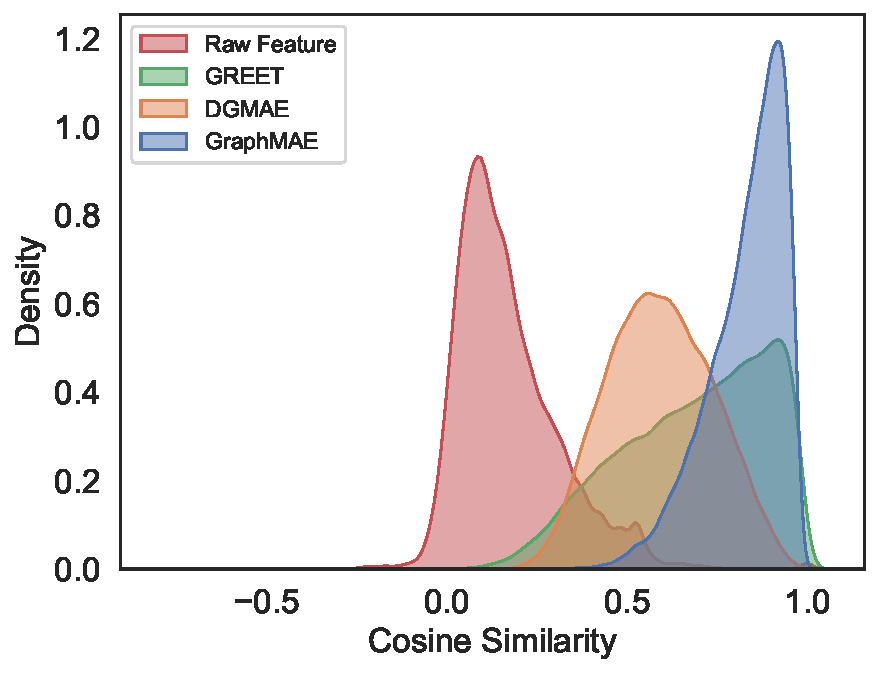
\includegraphics[height=0.40\textheight]{new_roman.pdf}\\[0.4em]
      {\scriptsize GraphMAE makes them similar ($\sim$1.0);\\ DGMAE preserves the discrepancy}
    \end{column}
  \end{columns}
  \ketluan{Attention \textbf{identifies heterophilic edges} $\Rightarrow$ DGMAE \textbf{preserves node discrepancy}}
  % Lời thoại:
  % - Số và hình trên slide này là của paper. Table 6 chỉ dùng L_d nên số thấp hơn Table 1; p_c = 0.2, p_τ = 1.
  % - Fig. 4 (ảnh hưởng của p_c): có lợi trên đồ thị dị tính, có hại trên đồ thị đồng tính.
  % - Fig. 8: cosine similarity của cặp node nối nhau nhưng khác lớp. GMAE đẩy similarity lên ~1.0 (đồng nhất hóa);
  %   DGMAE kéo về gần phân bố của đặc trưng gốc → giải quyết đúng vấn đề nêu ở Figure 2 phần mở đầu.
  % - (Tùy chọn, nếu nhóm kịp) vẽ lại Fig. 8 từ embedding của nhóm (train_node.py --save_emb).
  % - Fig. 5 (tỉ lệ che, Roman): DGMAE ổn định khi che tới 80%, GraphMAE giảm từ 46.73 xuống 38.2 — nói miệng nếu được hỏi.
\end{frame}

% ── Slide: Độ nhạy λ (Fig. 10) — 2 cột cân nhau: hình paper | hình nhóm, cùng kích thước ──
\begin{frame}{Sensitivity to $\lambda$}
  \begin{columns}[T]
    \begin{column}{0.48\textwidth}
      \centering
      {\small\textbf{Paper — Fig.~10}}\\[0.4em]
      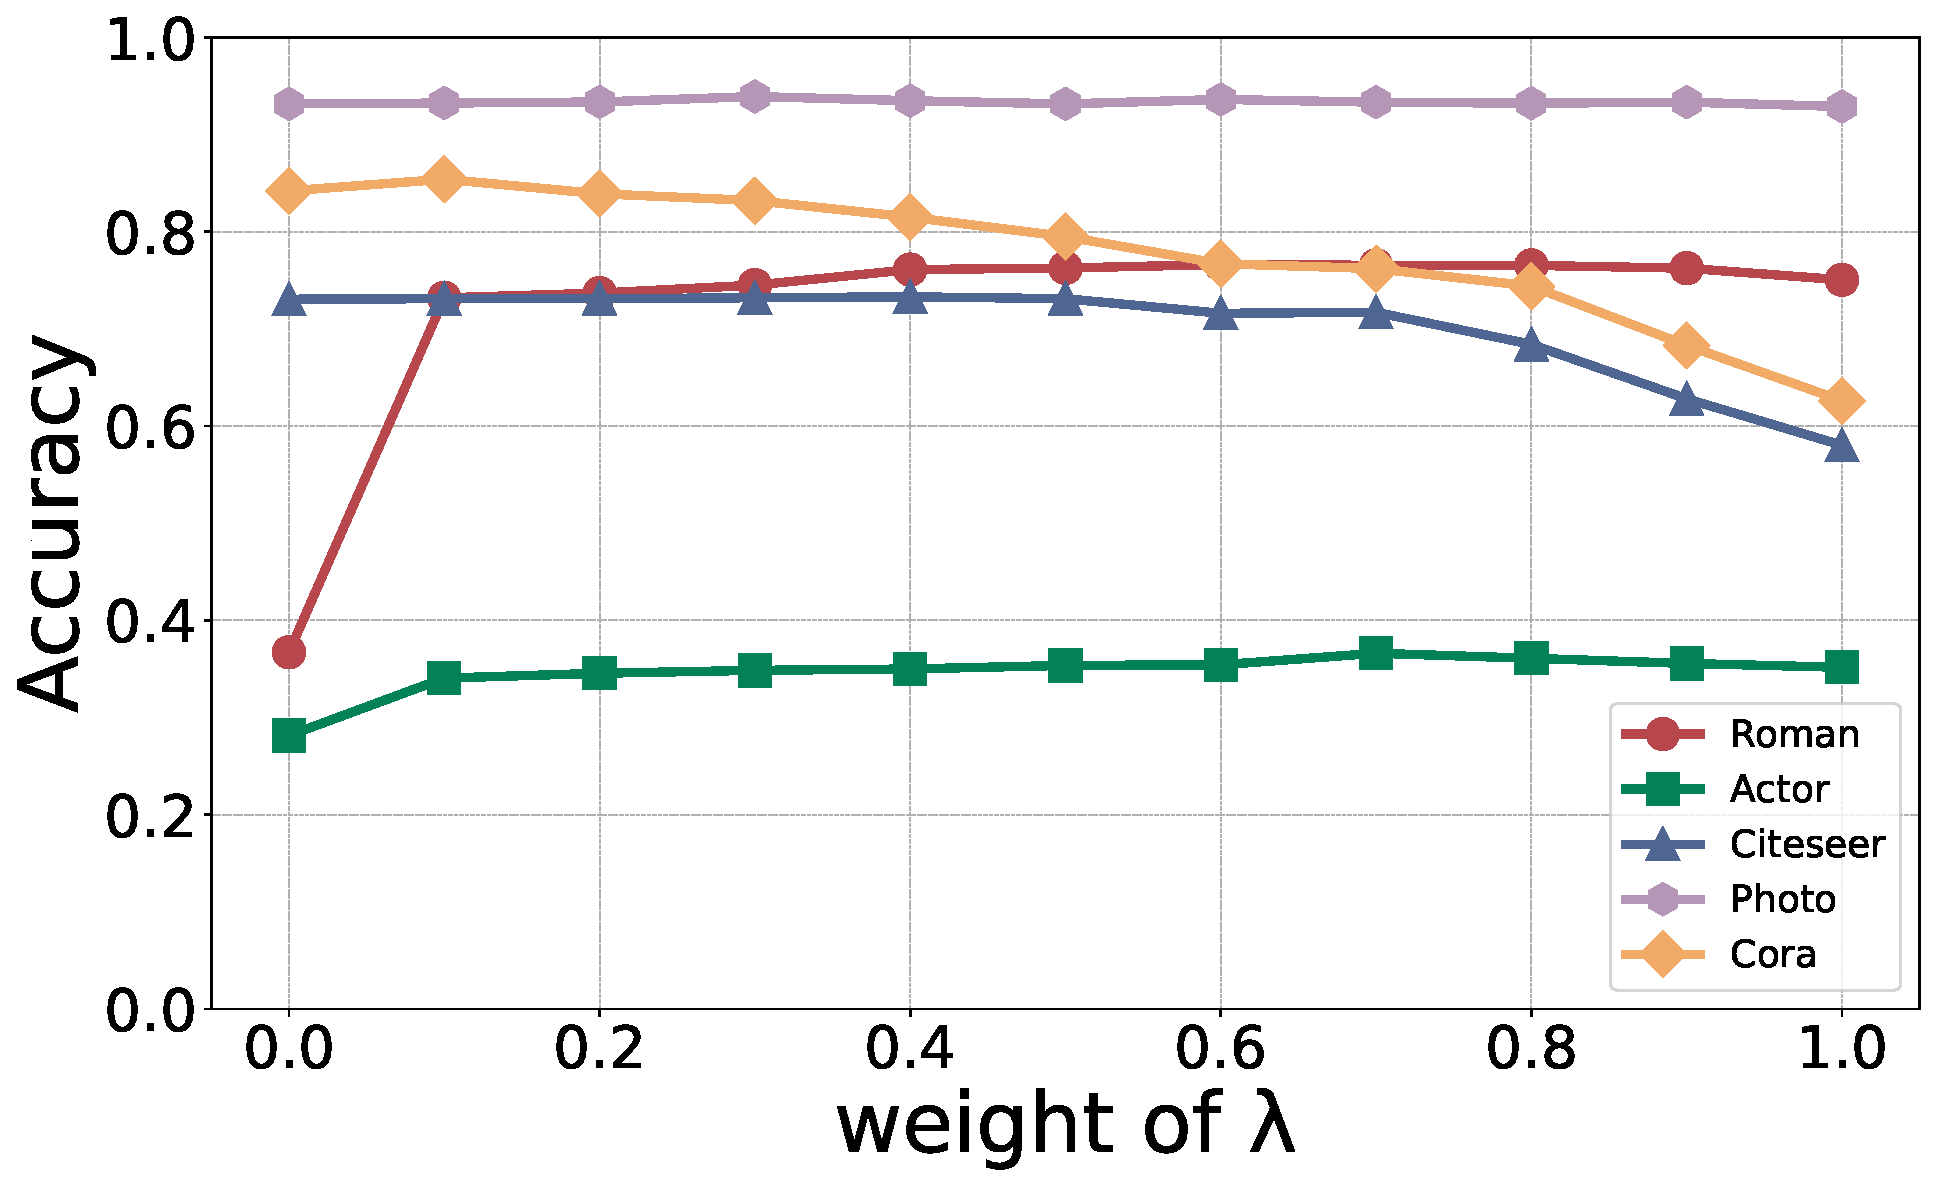
\includegraphics[height=0.45\textheight]{lambda_sens.pdf}
    \end{column}
    \begin{column}{0.48\textwidth}
      \centering
      {\small\textbf{\nh{Reproduced} — Cornell, Cora}}\\[0.4em]
      % Khi có kết quả: thay khung dưới bằng \includegraphics[height=0.45\textheight]{lambda_nhom.pdf}
      \hinhcho{0.85\linewidth}{0.45\textheight}{[ĐIỀN] Accuracy vs.\ $\lambda$\\ Cornell (heterophilic), Cora (homophilic)}
    \end{column}
  \end{columns}
  \ketluan{Paper: heterophilic graphs need large $\lambda$ (0.4--0.7), homophilic graphs small $\lambda$ ($\approx$0.1) · Reproduced: [ĐIỀN]}
  % Lời thoại:
  % - λ = 0: chỉ L_f (≈ GraphMAE); λ = 1: chỉ L_d.
  % - λ cần chọn theo mức độ dị tính của đồ thị — đây cũng là một hạn chế (thêm siêu tham số).
  % - Nhóm: [ĐIỀN]. Hình của nhóm: [ĐIỀN: script vẽ, ví dụ scripts/plot_lambda.py — chưa có].
\end{frame}

\section{Conclusion}

% ── Slide: Key findings ──────────────────────────────
\begin{frame}{Key Findings}
  \centering
  \renewcommand{\arraystretch}{1.4}
  \begin{tabular}{p{0.58\textwidth} p{0.30\textwidth}}
    \toprule
    \textbf{Finding (paper)} & \textbf{Reproduced?} \\
    \midrule
    DGMAE is best on \textbf{heterophilic graphs} (classification \& clustering) & \nh{[ĐIỀN]} \\
    \textbf{No loss} on homophilic graphs and graph classification         & \nh{[ĐIỀN]} \\
    $\mathcal{L}_d$ is the \textbf{key component} on heterophilic graphs  & \nh{[ĐIỀN]} \\
    $\lambda$ must be tuned to the heterophily level                       & \nh{[ĐIỀN]} \\
    \midrule
    \textbf{Overall reproducibility}                                        & \nh{[ĐIỀN]} \\
    \bottomrule
  \end{tabular}
  \ketluan{[ĐIỀN: một câu tổng kết — điều nhóm tin chắc nhất sau khi chạy lại]}
  % Lời thoại:
  % - Cột "Nhóm kiểm chứng": ghi ngắn, ví dụ "Có — 5/7 dataset" / "Một phần" / "Không" (điền theo số chính thức).
  % - Slide này trả lời trực tiếp yêu cầu "key findings" của đồ án.
\end{frame}

% ── Slide: Kết luận ──────────────────────────────────
\begin{frame}{Conclusion}
  \begin{itemize}
    \setlength{\itemsep}{1em}
    \item \textbf{Paper:} reconstructing the \textbf{discrepancy} $\Rightarrow$ clear gains on \textbf{heterophilic graphs},
      no loss on homophilic graphs.
    \item \textbf{Reproduction:} DGMAE re-implemented from the paper, without the authors' code. Result: [ĐIỀN: một câu tóm tắt mức độ tái lập]
    \item \textbf{Limitation:} extra hyper-parameters ($\lambda$, $p_c$, $p_\tau$, $\gamma_2$) tuned per dataset
      $\rightarrow$ future work: choose $\lambda$ \textbf{automatically} from the heterophily level.
  \end{itemize}
  \ketluan{\textbf{A simple idea that works on heterophilic graphs} — [ĐIỀN: nhận xét về tính tái lập]}
  % Lời thoại:
  % - Nhóm tái lập [ĐIỀN] tác vụ trên [ĐIỀN] dataset.
  % - Hạn chế khác của phương pháp: encoder chạy 2 lần mỗi vòng. Hướng khác: huấn luyện mini-batch cho đồ thị lớn.
  % - Hạn chế của nhóm: chưa chạy dataset lớn, chưa tái hiện Table 5, 10, 11, 12.
\end{frame}

% ── Slide cảm ơn nằm trong main.tex (\makethankyou) ──


% ── Slide cảm ơn kết thúc ──
\makethankyou

\end{document}
